\documentclass[12pt]{article}
\usepackage[utf8]{inputenc}
\usepackage[T1]{fontenc}
\usepackage[francais]{babel}
\usepackage{amsthm}
\usepackage{lmodern}
\usepackage{amsmath}
\usepackage{amsfonts}
\usepackage{pict2e}
\usepackage{listing}
\usepackage{url}
\usepackage{pdfpages}
\usepackage{hyperref}
\usepackage{listings}
\usepackage[DIV15]{typearea}
\title{Rapport sur l'état des armées}
\author{LYAZIDI Reda  \hspace*{1cm} OUDOT Maxime}
\date{\today}
\begin{document}
\maketitle
\tableofcontents

\newpage
\vspace*{8cm}
\begin{center} \section*{Introduction} \end{center}

Dans l'optique de pouvoir créer une armée de différents soldats équipés pouvant se combattre, il nous avait été demandé d'implémenter une suite de design pattern.
Différents choix d'implémentation se sont offerts à nous afin de concrétiser chacun des objectifs demandés.
Le présent rapport explique les choix qui furent fait et la logique qui nous a conduit à les faire, ainsi que les difficultés rencontrées lors de l'implémentation.

\newpage
\section{L'Existant}
\subsection{Description}
Il s'agit du code de base qui nous a été donné. Il est constitué d'une architecture de base sur les soldats.\\
L'existant repose sur \textbf{2} design patterns :
\begin{enumerate}
\item[\textbf{Decorator:}] Il modélise le fait pour un soldat d'être armé,
en effet, ainsi on obtient par exemple une classe SoldierWithSword contenant un Soldat, comme il est visible sur ce diagramme ci-joint.
\textbf{La décoration de l'objet représente l'armement du soldat}.

\includegraphics[scale=1]{../UML/Realdecorator}

En effet ce diagramme est simplifié mais le fonctionnement est le même,
pour le bouclier il y a une classe SoldierWithShield, et il est tout à fait 
possible de décorer à l'infini (SoldierWith...With...With...).
La décoration peut se représenter comme un arbre tel que chaque nœud(=soldat) a au plus un fils, la feuille est un simple soldat sans arme décrivant le type d'unité
(infanterie, cavalerie,...).
Le principal \textbf{défaut} est qu'on ne peut limiter la décoration,( par exemple un soldat avec n épées). De plus la méthode pour supprimer un équipement n'est pas triviale car il faut descendre dans la décoration jusqu'au bon niveau et enlever
le nœud concerné (le parent pointe vers le fils de son fils), cependant
hormis l'introspection il est impossible de savoir à quel arme correspond la décoration.

\item[\textbf{Proxy:}] Son rôle est de servir d'intermédiaire pour la gestion de
l'armement soit la décoration, le proxy est ArmedUnit représentant un soldat armé.
Ainsi la classe ArmedUnitSoldier possède un soldat et une liste d'armes,
cela assure qu'un soldat ne peut avoir \textbf{qu'une arme de chaque}.
L'avantage est que si d'autres types de soldats
sont rajoutés ou de nouvelles armes, ArmedUnitSoldier les gèrera sans changer le 
code. Le défaut est que si une nouvelle arme est implémentée, il faut absolument
implémentée la décoration de soldat correspondante (SoldierWith{Arme}).

Ainsi il est possible de créer/manipuler des soldats armés (ArmedUnit),
sans avoir à gérer la décoration, c'est seulement si l'on souhaite rajouter des nouvelles armes.
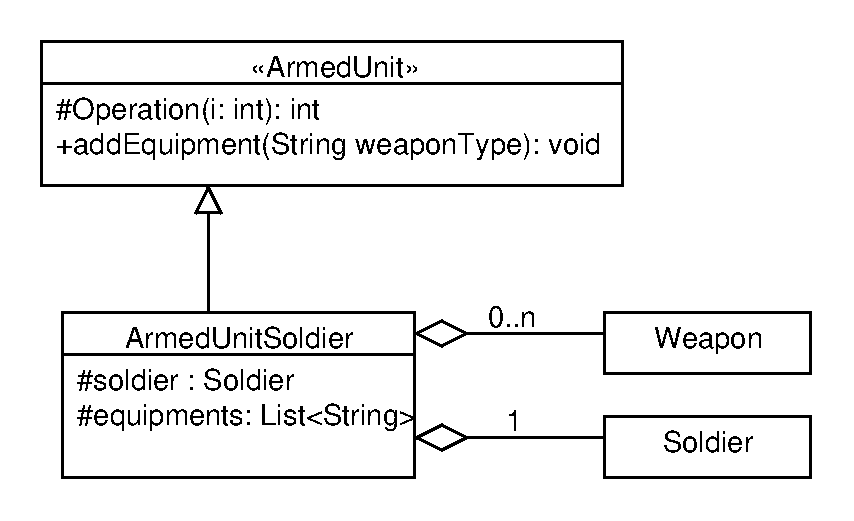
\includegraphics[scale=1]{../UML/Proxy}

Cependant rien n'empêche de surcharger une unité avec énormément d'armes.
\end{enumerate}
\subsection{Modifications apportées}
Dans le code de l'existant, la méthode "heal" soignait même si le soldat était mort (cela revenait à le ressusciter).
Dans le but de tests pour le \textbf{Composite}, il a été décidé d'implémenter \underline{\textbf{deux}} méthodes :
\begin{enumerate}
 \item \textbf{infuse\_life} étant la méthode "heal" de départ donc ressuscitant aussi;
 \item \textbf{heal} qui ne ressuscite pas et qui ne fonctionne donc que sur les soldats encore en vie.
\end{enumerate}

\newpage
\section{Implémentation}
\subsection{Composite}
Premier pattern que nous devions implémenter, il permet de \textbf{composer} une armée sans savoir son contenu.
Nous avons choisi de créer une interface Army, implémentée par Squadron, qui contient ainsi autant de sous-armées voulues, via ses soldats.

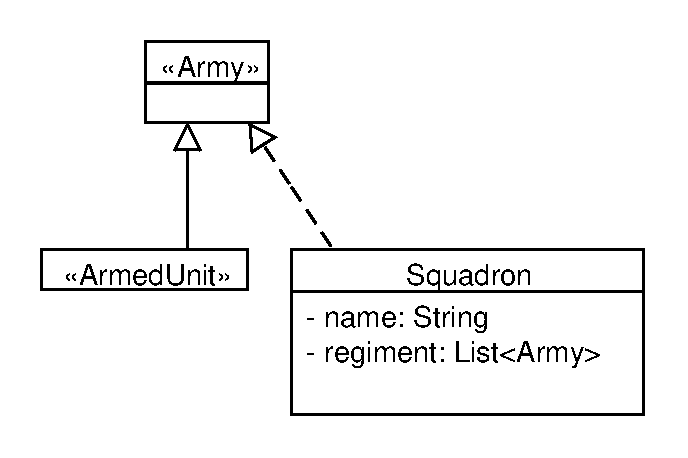
\includegraphics[scale=1]{../UML/Composite}

Ainsi une armée représente de 0 à \textbf{n} soldats.
Contrairement au decorator ici la structure de données pour représenter ce pattern
est un arbre (nombre de fils 0 à n, dont les feuilles sont les ArmedUnit.
Quel que soit la disposition des soldats dans le composite, l'armée inflige 
toujours autant de dégâts, soit la somme des soldats, il en va de même pour les 
points de vie.
Il est à noter qu'un bataillon (Squadron) ne gère que ses membres directs.
Soit dans un arbre chaque nœud ne s'occupe que de ses fils directs.
L'escadron répartit de manière équitable les dégâts entre ses membres.
Ainsi la répartition des dégâts se fait par nœud, donc selon la disposition
chaque unité ne subit pas le même nombre de dégâts.
Pour résumer chaque soldat du même escadron subit autant de dégâts que
ses frères et si l'un d'eux est un escadron il les répartit parmi à ses
fils.
Ainsi les dégâts qu'une unité subit dépend de 2 paramètre :
\begin{enumerate}
\item le nombre de d'armées dans l'escadron car plus il y a de membres plus
les dégâts sont divisés
\item son niveau dans la hiérarchie (l'arbre), car plus on en descend dans la
composition plus les dégâts on était dispersé parmi les autres armées.\\
La gestion de l'armement repose sur le principe du composite, on ajoute une arme
à une armée, si c'est un seul soldat alors on lui ajoute l'arme comme le fait le
proxy, si c'est un escadron alors on ajoute l'arme à chaque membre de l'escadron,
et comme il a été cité précédemment si une unité reçoit une arme qu'elle avait
déjà aucun changement (pour cette unité) a lieu.
Un défaut est qu'il est possible d'ajouter des armes à une armée vide,
bien qu'au final l'armée n'a pas les moyens de stocker l'arme donc aucune 
conséquence, mais la méthode n'est pas bloquante.

Une armée est morte quand \textbf{tous} ces soldats sont morts.
\end{enumerate}
\subsection{Visitor}
Le pattern Visitor, qui se couple très bien avec le précédent pattern, le pattern Composite, permet de \textbf{visiter} la composition créée par celui-çi. Celà permet de faire remonter une information sans connaître l'intérieur de la composition.
Nous devions ainsi implémenter deux traitements :
\begin{enumerate}
 \item l'affichage de tous les soldats formant un groupe armé;
 \item le comptage des soldats suivant leur type, au sein d'une armée.
\end{enumerate}
Pour cela, nous pensions d'abord créer une classe VisitorArmyCount qui compterait, pendant le parcours de l'armée, tout les types de soldats, en les stockant dans une Hashmap. Cependant, dans l'optique de ne pas risquer d'effets de bord (par exemple en utilisant plusieurs fois la même instance du visiteur) nous avons préféré utiliser la généricité. Il nous est alors possible de retourner différentes valeurs (telles que Integer et Void) lors du parcours, afin de remonter le nombre de soldats d'un type donné, alors passé en paramètre du visiteur.
\subsection{Observer}

\end{document}